% Copyright 2004 by Till Tantau <tantau@users.sourceforge.net>.
%
% In principle, this file can be redistributed and/or modified under
% the terms of the GNU Public License, version 2.
%
% However, this file is supposed to be a template to be modified
% for your own needs. For this reason, if you use this file as a
% template and not specifically distribute it as part of a another
% package/program, I grant the extra permission to freely copy and
% modify this file as you see fit and even to delete this copyright
% notice. 

% \UseRawInputEncoding
\documentclass{beamer}

% There are many different themes available for Beamer. A comprehensive
% list with examples is given here:
% http://deic.uab.es/~iblanes/beamer_gallery/index_by_theme.html
% You can uncomment the themes below if you would like to use a different
% one:
%\usetheme{AnnArbor}
%\usetheme{Antibes}
%\usetheme{Bergen}
%\usetheme{Berkeley}
%\usetheme{Berlin}
%\usetheme{Boadilla}
%\usetheme{boxes}
%\usetheme{CambridgeUS}
%\usetheme{Copenhagen}
%\usetheme{Darmstadt}
%\usetheme{default}
%\usetheme{Frankfurt}
%\usetheme{Goettingen}
%\usetheme{Hannover}
%\usetheme{Ilmenau}
%\usetheme{JuanLesPins}
%\usetheme{Luebeck}
\usetheme{Madrid}
%\usetheme{Malmoe}
%\usetheme{Marburg}
%\usetheme{Montpellier}
%\usetheme{PaloAlto}
%\usetheme{Pittsburgh}
%\usetheme{Rochester}
%\usetheme{Singapore}
%\usetheme{Szeged}
%\usetheme{Warsaw}

\usepackage{pgfgantt}
\usepackage{todonotes}
\usepackage{media9}
\usepackage{subfigure}
\usepackage{booktabs,array}


% Customize Warsaw color 
\setbeamercolor*{palette primary}{use=structure,fg=white,bg=red!50!black}
\setbeamercolor*{palette secondary}{use=structure,fg=white,bg=red!60!black}
\setbeamercolor*{palette tertiary}{use=structure,fg=white,bg=red!70!black}

% Customize Warsaw block title and background colors
\setbeamercolor{block title}{bg=red!50!black,fg=white}

\setbeamertemplate{bibliography item}{\insertbiblabel}  % insert bibliography numbers instead of symbol
\setbeamertemplate{caption}[numbered] % adds the figure or table number to the caption.

%==============================================================================
%     TITLE
%==============================================================================
\title[Smart Robotic Cart]{Smart Robotic Cart: A Prototype}

\author[K.~Allen, D.~Beebe, J.~Braker]{Kallistah~Allen \and Darrah~Beebe \and Jason~Braker
Advisors:~Dr.~Suruz~Miah \and Dr.~Prasad~Shastry}
% - Give the names in the same order as the appear in the paper.
% - Use the \inst{?} command only if the authors have different
%   affiliation.

\institute[Bradley University] % (optional, but mostly needed)
{
  Department of Electrical and Computer Engineering\\
  Bradley University\\
  1501 W. Bradley Avenue\\
  Peoria, IL, 61625, USA
}
% - Use the \inst command only if there are several affiliations.
% - Keep it simple, no one is interested in your street address.

\date[April~20,~2021]{Tuesday, April~20,~2021}

% - Either use conference name or its abbreviation.
% - Not really informative to the audience, more for people (including
%   yourself) who are reading the slides online

\logo{\hfill\href{http://www.bradley.edu}{
\includegraphics[width=0.75cm]{figs/logoBU1-Print}}}  % place logo in every page 


\subject{Mobile Robot Localization}
% This is only inserted into the PDF information catalog. Can be left
% out. 

% If you have a file called "university-logo-filename.xxx", where xxx
% is a graphic format that can be processed by latex or pdflatex,
% resp., then you can add a logo as follows:

% \pgfdeclareimage[height=0.5cm]{university-logo}{university-logo-filename}
% \logo{\pgfuseimage{university-logo}}

% Delete this, if you do not want the table of contents to pop up at
% the beginning of each subsection:
\AtBeginSection[]
{
  \begin{frame}<beamer>{Outline}
    \tableofcontents[currentsection,currentsubsection]
  \end{frame}
}

%==============================================================================
%==============================================================================
%     START OF SLIDES
%==============================================================================
%==============================================================================

% Let's get started
\begin{document}

\begin{frame}
  \titlepage
\end{frame}

\begin{frame}{Outline} 
  \tableofcontents%[pausesections]
  % You might wish to add the option [pausesections]
\end{frame}

% Section and subsections will appear in the presentation overview
% and table of contents.
\section{Introduction}

\begin{frame}{Introduction}{}
 \begin{center}
    \href{videos/proposalVideo.mp4}{
\includegraphics[width=0.8\textwidth]{figs/img/proposalVideoTitle}}
  \end{center}
\end{frame}

\begin{frame}{Problem Statement}
  \begin{block}{Problem Statement}
    \begin{LARGE}
      Design a robotic cart that follows the user.
    \end{LARGE}
  \end{block}
  \pause
  \begin{block}{Proposed Solution}
    \begin{LARGE}
      Utilize wireless signal strength to locate and then follow the user.
    \end{LARGE}
  \end{block}
\end{frame}

\begin{frame}{Existing Solutions}
  \begin{block}{Problems}
    \begin{itemize}
      \item Require line-of-sight between robot and user
      \item Some require costly dedicated image processing hardware
    \end{itemize}
  \end{block}
  \pause
  \begin{block}{Benefits of Proposed Solution}
    \begin{itemize}
      \item Line-of-sight is not required since analog RF signals will be used
      \item RF components are cost-effective
    \end{itemize}
  \end{block}
\end{frame}


\begin{frame}{System Requirements}
  \begin{block}{Specifications}
    \begin{itemize}
      \item Cart should be able to follow the remote target
      \item Cart should maintain a distance of 1~[\si{\meter}] to 1.5~[\si{\meter}] from the remote target.
      \item Cart should be able to attain a speed of at least 1~[\si{\meter\per\second}]
      \item Cart should not require line-of-sight to follow remote
     \end{itemize}
  \end{block}
\end{frame}


%------------------------------------------------------------------------------
%     SECTION BREAK
%------------------------------------------------------------------------------

\section{System Architecture}

\begin{frame}{System Components}
  \begin{block}{Main Components}
    \begin{itemize}
      \item Budget Bot mobile robot chassis (Fig. \ref{fig:budgetBotChassis})
      \item BeagleBone Blue (Fig. \ref{fig:beagleboneBlue})
      \item XBee S2C module (Fig. \ref{fig:XBeeModule})
    \end{itemize}
  \end{block}
  \begin{figure}
    \centering
    \begin{minipage}[t]{0.32\textwidth}
      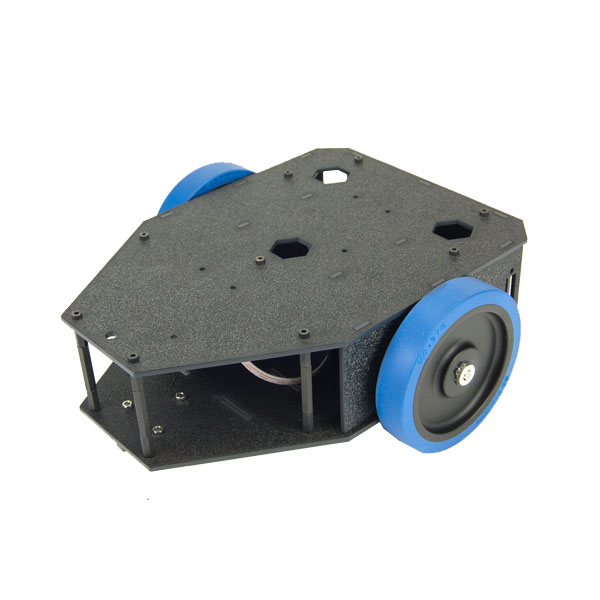
\includegraphics[width=1\textwidth]{figs/img/budgetbot_chassis}
      \caption{Budget Bot Chassis}
      \label{fig:budgetBotChassis}
    \end{minipage}%
    \begin{minipage}[t]{0.32\textwidth}
      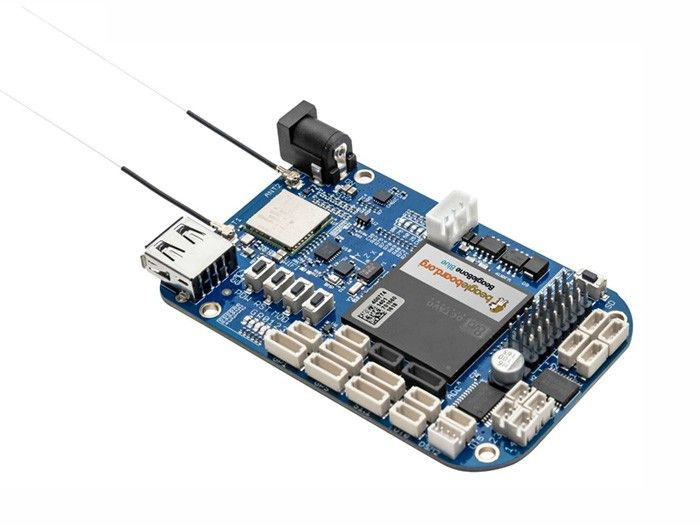
\includegraphics[width=1\textwidth]{figs/img/beaglebone_blue}
      \caption{BeagleBone Blue}
      \label{fig:beagleboneBlue}
    \end{minipage}
    \begin{minipage}[t]{0.32\textwidth}
      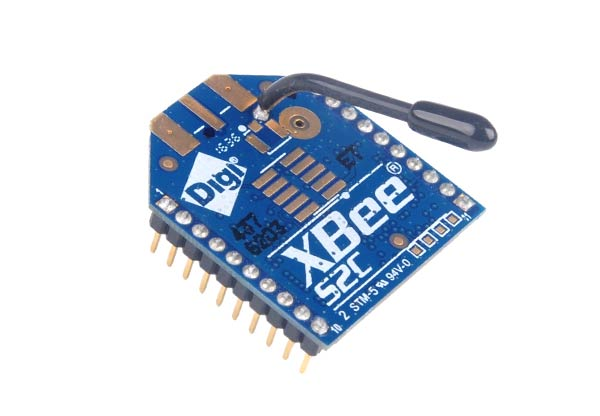
\includegraphics[width=1\textwidth]{figs/img/Xbee-S2C-Module}
      \caption{XBee S2C Module}
      \label{fig:XBeeModule}
    \end{minipage}
  \end{figure}
\end{frame} 

\begin{frame}{System Components}
    \begin{block}{Reflector Array}
    Two designs for reflector array:
    \begin{itemize}
      \item Paraboloidal Reflector (Fig. \ref{fig:parabolodialReflector})
      \item Combined Parabolic/Paraboloidal Reflector (Fig. \ref{fig:parabolicReflector})
    \end{itemize}
    \end{block}
    \begin{figure}
      \centering
      \begin{minipage}[t]{0.5\textwidth}
        \centering
        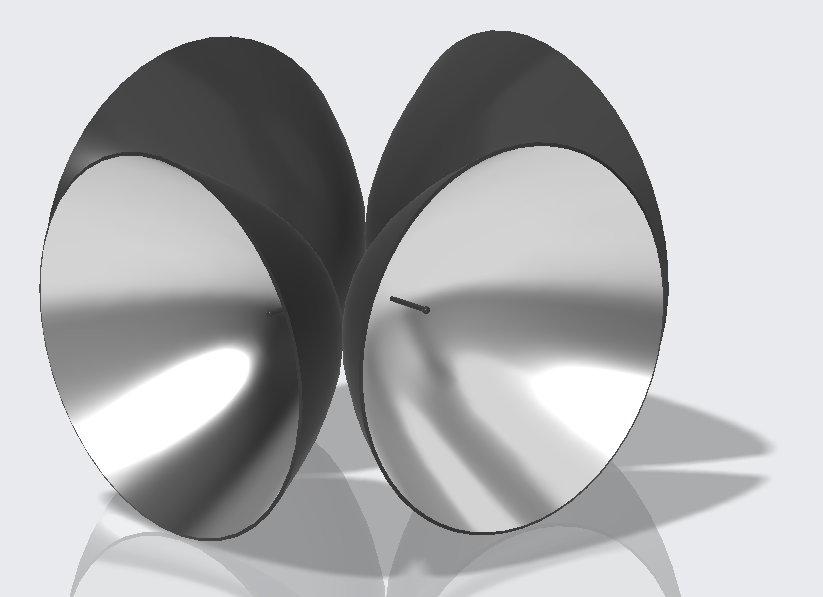
\includegraphics[height=3.5cm]{figs/img/paraboloidalReflector}
        \caption{Paraboloidal Reflector Model}
        \label{fig:parabolodialReflector}
      \end{minipage}
      \begin{minipage}[t]{0.4\textwidth}
        \centering
        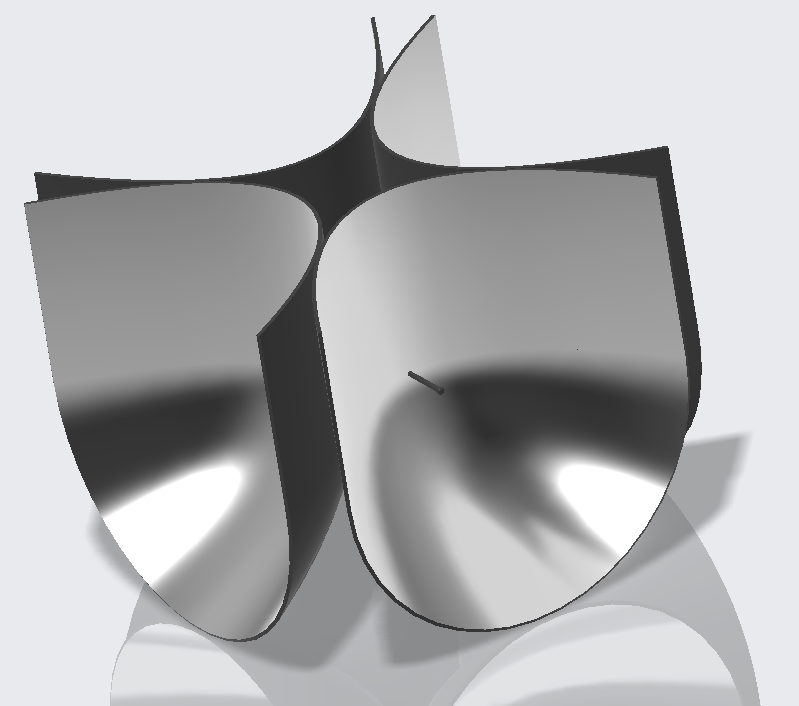
\includegraphics[height=3.5cm]{figs/img/parabolicReflector}
        \caption{Combined Parabolic/Paraboloidal Reflector}
        \label{fig:parabolicReflector}
      \end{minipage}
    \end{figure}
\end{frame}

\setlength{\dashlinedash}{2pt}
\setlength{\dashlinegap}{4pt}
\setlength{\arrayrulewidth}{0.3pt}

\begin{frame}{System Components}
  \begin{table}[h!]
      \centering
      \begin{tabular}{c|c}
          \toprule
          \textbf{Quantity} & \textbf{Parts}\\
          \toprule
          2 & Budget Bot Chassis\\
          2 & Battery Packs for Budget Bot\\ \hdashline
          4 & 10 uF Ceramic Capacitor\\
          4 & LM1117 Regulator\\
          8 & 9V Batteries\\
          4 & Solderable PCB Boards\\ \hdashline
          3 & XBee USB Adapter\\
          \bottomrule
          %\multicolumn{2}{r|}{\textbf{Total}} & \$ 562.34\\
          %\bottomrule
      \end{tabular}
      \caption{Parts Available in Laboratory}
      \label{tab:Partslablist}
  \end{table}
\end{frame}

\begin{frame}{System Components}
  \begin{table}[h!]
    \centering
    \begin{tabular}{c|c|c}
      \toprule
      \textbf{Quantity} & \textbf{Parts} & \textbf{Price}\\
      \toprule
      12 & XBee S2C Module & \$ 23.10\\
      10 & XBee Adapter Board & \$ 4.99\\ \cdashline{1-2}
      4 & Pololu 37D Metal Gearmotor 4751 & \$ 39.95\\
      2 & Twotrees 4 Lead Nema 17 Stepper Motor & \$ 9.99\\ \cdashline{1-2}
      1 & 4-Pin JST SH Connector - 20 Pack & \$ 7.99\\
      1 & 6-Pin JST SH Connector - 10 Pack & \$ 9.99\\ \cdashline{1-2}
      1 & Aluminum Foil Tape - 2 in x 5 yd & \$ 6.05\\
      \bottomrule
      \multicolumn{2}{r|}{\textbf{Total}} & \$ 562.34\\
      \bottomrule
    \end{tabular}
    \caption{Purchased parts for the Robotic Cart Project}
    \label{tab:Partslist}
  \end{table}
\end{frame}
 

%------------------------------------------------------------------------------
%     SECTION BREAK
%------------------------------------------------------------------------------

\section{Customized Reflector Array}

\begin{frame}{Customized Reflector Array}
  
\end{frame}

%------------------------------------------------------------------------------
%     SECTION BREAK
%------------------------------------------------------------------------------

\section{Algorithms}

\begin{frame}{Algorithms}
  
\end{frame}

%------------------------------------------------------------------------------
%     SECTION BREAK
%------------------------------------------------------------------------------

\section{Implementation}

\begin{frame}{Implementation}
  
\end{frame}

%------------------------------------------------------------------------------
%     SECTION BREAK
%------------------------------------------------------------------------------

\section{Conclusion and Future Work}

\begin{frame}{Conclusion and Future Work}
  
\end{frame}

%==============================================================================
%==============================================================================
%     END OF SLIDES
%==============================================================================
%==============================================================================

% \subsection*{Demonstration}

% \begin{frame}{Demonstration}
%     \centering
%     \includemedia[
%      width=0.8\linewidth,
%      height=0.6\linewidth,
%      activate=pageopen,  
%      addresource=videos/Demonstration_Trim.mp4,
%      flashvars={
%       source=videos/Demonstration_Trim.mp4
%       &loop=true  % loop the video
%      }
%     ]{}{VPlayer.swf}
% \end{frame}

%----------------------------------

% \begin{frame}{Introduction}{}
% \begin{figure}
%   \centering
%   \includegraphics[scale=0.31]{figs/ipe/highLevel_wht_grn}
%   \caption{General high-level system architecture}
%   \label{fig:ProblemStatementImage}
% \end{figure}
% \end{frame}

% \begin{frame}{Introduction}{}
%         \begin{itemize}
%         \item This project will:
%             \begin{itemize}
%                 \item use a pair of 2-DOF (2-degrees-of-freedom) mechatronics platforms
%                 \item implement control algorithms on embedded system
%                 \item use mobile device for user control
%                 \item encourage research
%                 \item serve as an educational tool
%             \end{itemize}
%         \end{itemize}
% \end{frame}

% %----------------------------------

% \section{Background Study}

% \subsection{Control Techniques}

% \begin{frame}{Background Study}{Control Techniques}
%     Various control techniques have been proposed for 2-DOF helicopters such as:
%     \begin{itemize}
%         \item Sliding mode control \cite{Ahmed2010-Sliding} %cite 2-Sliding Mode Based Robust Control for 2-DOF Helicopter here
%         \item Fuzzy Logic control 
%         \cite{Chang2017-Fuzzy}
%         \cite{Kayacan2016-Fuzzy}
%         \cite{Mendez-Monroy2012-Fuzzy} 
%         %cite Fuzzy control with estimated variable sampling period for non-linear networked control systems: 2-DOF helicopter as case study here
%         \item Data-driven Adaptive Optimal Output-feedback control \cite{Gao2016-DataDriven} %cite Data-driven Adaptive Optimal Output-feedback Control of a 2-DOF Helicopter here
%         \item Decentralized discrete-time neural control \cite{Hernandez-Gonzalez2012-Decentralized} %cite Decentralized discrete-time neural control for a Quanser 2-DOF helicopter here
%     \end{itemize}
%     These control techniques employ advanced mathematics that are difficult to implement on embedded systems.
% \end{frame}

% %----------------------------------

% \subsection{Modeling a 2-DOF Helicopter}

% \begin{frame}{Background Study}{Modeling a 2-DOF Helicopter}
%     \begin{columns}
%     \column{0.5\textwidth}
%     \begin{figure}
%         \centering
%         \includegraphics[width=\textwidth]{figs/img/helicopterModel}
%         \caption{Model of a 2-DOF helicopter}
%         \label{fig:helicopterModel}
%     \end{figure}
%     \column{0.5\textwidth}
%     \begin{figure}
%       \centering 
%       \includegraphics[width=\textwidth]{figs/img/QuanserAero}
%       \caption{Quanser Aero}
%       \label{fig:QuanserAero}
%     \end{figure}    
%     \end{columns}
% \end{frame}

% \begin{frame}{Background Study}{Modeling a 2-DOF Helicopter}
%     \begin{itemize}
%         \item Characterized by fixed base
%         \begin{itemize}
%             \item Can change 2 of 3 possible orientations...
%             \begin{itemize}
%                 \item Pitch ($\theta$)
%                 \item Yaw ($\psi$)
%                 \item \emph{Not Roll}
%             \end{itemize}
%             \item and cannot change position
%             \begin{itemize}
%                 \item x direction
%                 \item y direction
%                 \item z direction
%             \end{itemize}
%         \end{itemize} 
%     \end{itemize}
% \end{frame}

% % \begin{frame}{Background Study}{Quanser Aero} 

% % \end{frame}

% \begin{frame}{Background Study}{Modeling a 2-DOF Helicopter}
%     \begin{itemize}
%         \item Motors are attached to the propellers to create thrust due to air resistance
%             \begin{itemize}
%                 \item Main - changes pitch angle
%                 \item Tail - changes yaw angle
%             \end{itemize} 
%         \item Torque due to rotation also creates a force on opposite axes 
%     \end{itemize}
% \end{frame}

% \begin{frame}{Background Study}{Modeling a 2-DOF Helicopter}
% Due to the efficiency of the Quanser Aero, we can create a linearized system model:
% \begin{align}
%   %\dot{\bf x}(t) = {\bf A}{\bf x}(t) +{\bf B}{\bf u}(t),~\mathrm{where}
%     \dot{\bf x}(t) = {\bf A}{\bf x}(t) +{\bf B}{\bf u}(t),~\mathrm{such}~\mathrm{that}
% \label{eq:stateModel}
% \end{align}  
% %
% \begin{align*}
% \begin{bmatrix}
%     \dot\theta\\
%     \dot\psi\\
%     \ddot{\theta}\\
%     \ddot{\psi}
% \end{bmatrix}&=
% %\label{eq:matrixA}
% \begin{bmatrix}
%     0 & 0 & 1 & 0 \\
%     0 & 0 & 0 & 1 \\
%     0 & -K_{sp}/J_p & -D_p/J_p & 0 \\
%     0 & 0 & 1 & -D_y/J_y 
% \end{bmatrix} 
% %\label{eq:stateMatrix} 
% \begin{bmatrix}
%     \theta\\
%     \psi\\
%     \dot{\theta}\\
%     \dot{\psi}
% \end{bmatrix}
% \\&+
% %\label{eq:matrixB}
% \begin{bmatrix}
%     0 & 0 \\
%     0 & 0 \\
%     K_{pp}/J_p & K_{py}/J_p \\
%     K_{yp}/J_y & K_{yy}/J_y 
% \end{bmatrix}
% %\label{eq:inputMatrix}
% \begin{bmatrix}
%     V_p \\
%     V_y 
% \end{bmatrix}
% %{\bf A} =  
% %\begin{bmatrix}
% %0 & 0 & 1 & 0\\
% %0 & 0 & 0 & 1\\
% %-\frac{K_{\text{sp}}}{J_p} & 0 & -\frac{D_p}{J_p} &  0\\
% %0 & 0 & 0 & -\frac{D_y}{J_y}    
% %\end{bmatrix}
% %~\text{and}~
% %  {\bf B} =
% %\begin{bmatrix}
% %0 & 0\\
% %0 & 0\\
% %\frac{K_{\text{pp}}}{J_p} & \frac{K_{\text{py}}}{J_p}\\
% %\frac{K_{\text{yp}}}{J_y} & \frac{K_{\text{yy}}}{J_y}                           
% %\end{bmatrix}
% \end{align*}
% \end{frame}

% \begin{frame}{Background Study}{Modeling a 2-DOF Helicopter}
% \begin{itemize}
%     \item $K_{sp}$ - being the stiffness of the axes
%     \item $K_{pp}$ - pitch motor thrust constant
%     \item $K_{py}$ - thrust constant acting on the pitch angle from the yaw motor
%     \item $K_{yp}$ - thrust constant acting on the yaw angle from the pitch motor
%     \item $K_{yy}$ - yaw motor thrust constant
%     \item $J_p$ - moment of inertia about pitch axis
%     \item $J_y$ - moment of inertia about yaw axis
%     \item $D_p$ - viscous damping of the pitch axis
%     \item $D_y$ - viscous damping of the yaw axis
% \end{itemize}
% \end{frame}

% %----------------------------------
% \subsection{Control Algorithm and Architecture}
% \begin{frame}{Background Study}{Control Algorithm Overview - Optimal Control}
% \begin{enumerate}
%     \item Employ state-space representation of 2-DOF helicopter:
%     \begin{align*}
%         \dot{\mathbf{x}} = \mathbf{A}\mathbf{x} + \mathbf{B}\mathbf{u}
%     \end{align*}
%     \item Use state feedback law
%     \begin{center}
%         $\mathbf{u} = -\mathbf{K}\mathbf{x}$
%     \end{center}
%     to minimize the quadratic cost function:
%     \begin{align*}
%         J(\mathbf{u}) = \int_0^\infty (\mathbf{x}^T\mathbf{Q}\mathbf{x} + \mathbf{u}^T\mathbf{R}\mathbf{u} + 2\mathbf{x}^T\mathbf{N}\mathbf{u})\mathrm{dt}
%     \end{align*}
%     \item Find the solution $\mathbf{S}$ to the Riccati equation
%     \begin{align*}
%         \mathbf{A}^T\mathbf{S}+\mathbf{SA}-(\mathbf{SB}+\mathbf{N})\mathbf{R}^{-1}(\mathbf{B}^T\mathbf{S}+\mathbf{N}^T)+\mathbf{Q}=0
%     \end{align*}    
%     \item Calculate gain, $\mathbf{K}$
%     \begin{center}
%         $\mathbf{K}=\mathbf{R}^{-1}(\mathbf{B}^T\mathbf{S}+\mathbf{N}^T)$
%     \end{center}
% \end{enumerate}
% \end{frame}
% %----------------------------------
% \begin{frame}{Background Study}{Control Algorithm Overview - Optimal Noise Resistant Control}
% \begin{itemize}
%     \item Utilizes gain calculated in LQR
%     \item Added Kalman filter to reduce external disturbances to the system
% \end{itemize} 
% \begin{figure}
%     \centering
%     \includegraphics[width=.8\textwidth,keepaspectratio=true]{figs/img/LQG_SimulinkResize.png}
%     \caption{Noise resistant 2-DOF helicopter model}
%     \label{fig:LQGModel}
% \end{figure}
% \end{frame}
% %----------------------------------
% \begin{frame}{Background Study}{Control Algorithm Overview - Machine Learning}
%     \begin{columns}
%     \column{0.5\textwidth}
%     \begin{figure}
%         \centering
%         \includegraphics[width=\textwidth]{figs/ipe/ADP_Neural_Network}
%         \caption{Neural network}
%         \label{fig:ADP_Neural_Networkl}
%     \end{figure}
%     \column{0.5\textwidth}
%     \begin{figure}
%       \centering 
%       \includegraphics[width=\textwidth]{figs/ipe/ADP_Samples}
%       \caption{Neural network sampling}
%       \label{fig:ADP_Samples}
%     \end{figure}    
%     \end{columns}
% \end{frame}
% %----------------------------------
% \begin{frame}{Background Study}{Control Architecture Overview -  P Type Controller}
% \begin{figure}
%     \centering
%     \includegraphics[width=.8\textwidth,keepaspectratio=true]{figs/ipe/P_Control}
%     \caption{Optimal P type controller [servo]}
%     \label{fig:P_Control}
% \end{figure}
% \end{frame}
% %----------------------------------
% \begin{frame}{Background Study}{Control Architecture Overview - PI Type Controller}
% \begin{figure}
%     \centering
%     \includegraphics[width=.8\textwidth,keepaspectratio=true]{figs/ipe/PI_Control}
%     \caption{Optimal PI type controller [servo]}
%     \label{fig:PI_Control}
% \end{figure}
% \end{frame}
% %----------------------------------

% \subsection{Prior Work}

% \begin{frame}{Background Study}{Prior Work}
%   \begin{itemize}
%       \item extensive modeling \& simulations
%       \item implementation of two motion control algorithms (LQR \& ADP)
%       \item one helicopter
%       %\item deployed on mobile device
%   \end{itemize}
% \end{frame}

% %----------------------------------

% % \subsection{Challenges}

% % \begin{frame}{Background Study}{Challenges}
  
% % \end{frame}

% %----------------------------------

% \section{Subsystem Level Functional Requirements}

% % put a slide with three dimensional system architecture drawing using ipe
% % another slide with explanation

% % put a slide with system block diagram

% \subsection{Block Diagram}

% \begin{frame}{Subsystem Level Functional Requirements}{Block Diagram}

% \begin{figure}
%   \centering
%   \includegraphics[scale=0.31]{figs/ipe/TCPModel}
%   \caption{Communication model}
%   \label{fig:TCPModel}
% \end{figure}

% \end{frame}

% \begin{frame}{Subsystem Level Functional Requirements}{Block Diagram} 

% \begin{figure}
%   \centering 
%   \includegraphics[scale=0.31]{figs/ipe/lowLevel}
%   \caption{Low level smart control diagram}
%   \label{fig:ProposalImage}
% \end{figure}

% \end{frame}

% %----------------------------------

% \section{Simulation}

% \subsection{Optimal Control Simulation}

% % P Controller
% \begin{frame}{Simulation}{Optimal Control Simulation (P Type Controller)}
%     \begin{figure}
%       \centering
%       \subfigure[][]{
%         \label{fig:LQR_Pos_Con}
%         \includegraphics[scale=0.38]{figs/MATLAB/LQR/P_Simulation/LQR_Pos_Con}
%       }
%       \subfigure[][]{
%         \label{fig:LQR_Volt_Con}
%         \includegraphics[scale=0.38]{figs/MATLAB/LQR/P_Simulation/LQR_Volt_Con}    
%       }  
%       \caption{Optimal control (P type controller) simulation \subref{fig:LQR_Pos_Con}~position and~\subref{fig:LQR_Volt_Con}~voltage w/ step input}
%       \label{fig:LQR_Sim_Con}
%     \end{figure}
% \end{frame}

% \begin{frame}{Simulation}{Optimal Control Simulation (P Type Controller)}
%     \begin{figure}
%       \centering 
%       \includegraphics[scale=0.5]{figs/MATLAB/LQR/P_Simulation/LQR_Error_Con}
%       \caption{Optimal control (P type controller) simulation w/ constant signal}
%       \label{fig:LQR_Error_Con}
%     \end{figure}
% \end{frame}

% % PI LQR vs LQG
% \subsection{Noise Resistant and Optimal Control Simulation}
% \begin{frame}{Simulation}{Noise Resistant and Optimal Control (PI type Controller) Simulation}
%     \begin{figure}
%       \centering
%       \subfigure[][]{
%         \label{fig:Pitch}
%         \includegraphics[scale=0.38]{figs/matlab/LQG_PIvLQR_PI_Sim/Pitch}
%       }
%       \subfigure[][]{
%         \label{fig:Yaw}
%         \includegraphics[scale=0.38]{figs/matlab/LQG_PIvLQR_PI_Sim/Yaw}    
%       }  
%       \caption{Noise resistant control vs optimal control (PI type controller) simulation \subref{fig:Pitch}~pitch~position and~\subref{fig:Yaw}~yaw~position w/ step input}
%       \label{fig:LQR_LQG_Sim_pos}
%     \end{figure}
% \end{frame}

% \begin{frame}{Simulation}{Noise Resistant and Optimal Control (PI Type Controller) Simulation}
%     \begin{figure}
%       \centering
%       \subfigure[][]{
%         \label{fig:Pitch_Volt}
%         \includegraphics[scale=0.38]{figs/matlab/LQG_PIvLQR_PI_Sim/Pitch_Volt}
%       }
%       \subfigure[][]{
%         \label{fig:Yaw_Volt}
%         \includegraphics[scale=0.38]{figs/matlab/LQG_PIvLQR_PI_Sim/Yaw_Volt}    
%       }  
%       \caption{Noise resistant control vs optimal control (PI type controller) simulation \subref{fig:Pitch_Volt}~pitch~voltage and~\subref{fig:Yaw_Volt}~yaw~voltage w/ step input}
%       \label{fig:LQR_PI_Sim_volt}
%     \end{figure}
% \end{frame}

% %% PI Controller
% %\begin{frame}{Simulation}{Optimal Control Simulation (PI Controller)}
% %    \begin{figure}
% %      \centering
% %      \subfigure[][]{
% %        \label{fig:Pitch_LQR_Sim}
% %        \includegraphics[scale=0.38]{figs/MATLAB/LQR/PI_Sim/Pitch_LQR_Sim}
% %      }
% %      \subfigure[][]{
% %        \label{fig:Yaw_LQR_Sim}
% %        \includegraphics[scale=0.38]{figs/MATLAB/LQR/PI_Sim/Yaw_LQR_Sim}    
% %      }  
% %      \caption{Optimal Control (PI Controller) Simulation \subref{fig:Pitch_LQR_Sim}~Pitch~Position and~\subref{fig:Yaw_LQR_Sim}~Yaw~Position w/ Step Input}
% %      \label{fig:LQR_PI_Sim_pos}
% %    \end{figure}
% %\end{frame}
% %
% %\begin{frame}{Simulation}{Optimal Control (PI Controller) Simulation}
% %    \begin{figure}
% %      \centering
% %      \subfigure[][]{
% %        \label{fig:Pitch_Volt_LQR_Sim}
% %        \includegraphics[scale=0.38]{figs/MATLAB/LQR/PI_Sim/Pitch_Volt_LQR_Sim}
% %      }
% %      \subfigure[][]{
% %        \label{fig:Yaw_Volt_LQR_Sim}
% %        \includegraphics[scale=0.38]{figs/MATLAB/LQR/PI_Sim/Yaw_Volt_LQR_Sim}    
% %      }  
% %      \caption{Optimal Control (PI Controller) Simulation \subref{fig:Pitch_Volt_LQR_Sim}~Pitch~Voltage and~\subref{fig:Yaw_Volt_LQR_Sim}~Yaw~Voltage w/ Step Input}
% %      \label{fig:LQR_PI_Sim_volt}
% %    \end{figure}
% %\end{frame}
% %
% %% LQG
% %\subsection{Optimal Noise Resistant Control Simulation}
% %\begin{frame}{Simulation}{Optimal Noise Resistant Control (PI Controller) Simulation}
% %    \begin{figure}
% %      \centering
% %      \subfigure[][]{
% %        \label{fig:Pitch_LQG_Sim}
% %        \includegraphics[scale=0.38]{figs/MATLAB/LQG/LQG_Sim/Pitch_LQG_Sim}
% %      }
% %      \subfigure[][]{
% %        \label{fig:Yaw_LQG_Sim}
% %        \includegraphics[scale=0.38]{figs/MATLAB/LQG/LQG_Sim/Yaw_LQG_Sim}    
% %      }  
% %      \caption{Optimal Noise Resistant Control (PI Controller) \subref{fig:Pitch_LQG_Sim}~Pitch~Position and~\subref{fig:Yaw_LQG_Sim}~Yaw~Position w/ Step Input}
% %      \label{fig:LQG_PI_Sim_pos}
% %    \end{figure}
% %\end{frame}
% %
% %\begin{frame}{Simulation}{Optimal Noise Resistant Control (PI Controller) Simulation}
% %    \begin{figure}
% %      \centering
% %      \subfigure[][]{
% %        \label{fig:Pitch_Volt_LQG_Sim}
% %        \includegraphics[scale=0.38]{figs/MATLAB/LQG/LQG_Sim/Pitch_Volt_LQG_Sim}
% %      }
% %      \subfigure[][]{
% %        \label{fig:Yaw_Volt_LQG_Sim}
% %        \includegraphics[scale=0.38]{figs/MATLAB/LQG/LQG_Sim/Yaw_Volt_LQG_Sim}    
% %      }  
% %      \caption{Optimal Noise Resistant Control Simulation (PI Controller) \subref{fig:Pitch_Volt_LQG_Sim}~Pitch~Voltage and~\subref{fig:Yaw_Volt_LQG_Sim}~Yaw~Voltage w/ Step Input}
% %      \label{fig:LQG_PI_Sim_volt}
% %    \end{figure}
% %\end{frame}

% %----------------------------------

% \section{Implementation}

% \subsection{USB}
% %LQR
% \begin{frame}{Implementation}{Optimal Control P and PI Type Controller USB}
%     \begin{figure}
%       \centering
%       \subfigure[][]{
%         \label{fig:Pitch_LQR_RMSE}
%         \includegraphics[scale=0.38]{figs/matlab/LQR_PIvLQR_P_USB/step/Pitch_LQR_RMSE}
%       }
%       \subfigure[][]{
%         \label{fig:Yaw_LQR_RMSE}
%         \includegraphics[scale=0.38]{figs/matlab/LQR_PIvLQR_P_USB/step/Yaw_LQR_RMSE}    
%       }  
%       \caption{USB implementation comparison between optimal control (P~type~controller) and optimal control (PI~type~controller) for \subref{fig:Pitch_LQR_RMSE}~pitch and \subref{fig:Yaw_LQR_RMSE}~yaw configurations w/ step input}
%       \label{fig:PvPI_USB}
%     \end{figure}
% \end{frame}
% %
% \begin{frame}{Implementation}{Optimal Control P and PI Type Controller USB}
%     \begin{figure}
%       \centering
%       \subfigure[][]{
%         \label{fig:PitchVoltage_LQR_RMSE}
%         \includegraphics[scale=0.38]{figs/matlab/LQR_PIvLQR_P_USB/step/PitchVoltage_LQR_RMSE}
%       }
%       \subfigure[][]{
%         \label{fig:YawVoltage_LQR_RMSE}
%         \includegraphics[scale=0.38]{figs/matlab/LQR_PIvLQR_P_USB/step/YawVoltage_LQR_RMSE}    
%       }  
%       \caption{USB implementation comparison between optimal control (P~type~controller) and optimal control (PI~type~controller) for \subref{fig:PitchVoltage_LQR_RMSE}~pitch and \subref{fig:YawVoltage_LQR_RMSE}~yaw voltages w/ step input}
%       \label{fig:PvPIVoltage_USB}
%     \end{figure}
% \end{frame}
% %
% \begin{frame}{Implementation}{Optimal Control P and PI Type Controller USB}
% \begin{table}
%     \centering
%     \begin{tabular}{l|l|l}
%         \toprule
%         \textbf{} & \textbf{Pitch Step} & \textbf{Yaw Step}\\
%         \toprule
%         LQR P & 3.5025 & 5.8502\\
%         LQR PI & 1.2349 & 5.5058\\
%         Improvement & 64.7437\% & 0.5408\% \\
%         \toprule
%         \textbf{} & \textbf{Pitch Square} & \textbf{Yaw Square}\\
%         \toprule
%         LQR P & 6.2819 & 20.4623\\
%         LQR PI & 6.9206 & 21.0709\\
%         Improvement & -10.1675\% & -2.9740\% \\
%         \toprule
%         \textbf{} & \textbf{Pitch Sine} & \textbf{Yaw Sine}\\
%         \toprule
%         LQR P & 4.2469 & 2.8644\\
%         LQR PI & 1.3383 & 1.7852\\
%         Improvement & 68.4872\% & 63.2998\% \\
%     \end{tabular}
%     \caption{Root mean squared error}
%     \label{tab:RMSE}
% \end{table}
% \end{frame}
% %\begin{frame}{Implementation}{Optimal Control P and PI Controller USB}
% %\begin{table}
% %    \centering
% %    \begin{tabular}{l|l|l|l|l|l|l}
% %        \toprule
% %        \textbf{0} & \textbf{Pitch Step} & \textbf{Yaw Step} & \textbf{Pitch Square} & \textbf{Yaw Square} & \textbf{Pitch Sine} & \textbf{Yaw Sine}\\
% %        \toprule
% %        LQR P & 3.5025 & 5.8502 & 6.2819 & 20.4623 & 4.2469 & 2.8644\\
% %        LQR PI & 1.2349 & 5.5058 & 6.9206 & 21.0709 & 1.3383 & 1.7852
% %        \bottomrule
% %    \end{tabular}
% %    \caption{Root Mean Squared Error}
% %    \label{tab:RMSE}
% %\end{table}
% %\end{frame}
% %Machine vs LQR
% \begin{frame}{Implementation}{Machine Learning and Optimal Control (P Type Controller) USB}
%     \begin{figure}
%       \centering
%       \subfigure[][]{
%         \label{fig:Pitch_LQRvADP_USB}
%         \includegraphics[scale=0.38]{figs/matlab/ADPvLQR_P_USB/Pitch_ADP_LQR}
%       }
%       \subfigure[][]{
%         \label{fig:Yaw_LQRvADP_USB}
%         \includegraphics[scale=0.38]{figs/matlab/ADPvLQR_P_USB/Yaw_ADP_LQR}    
%       }  
%       \caption{USB implementation comparison between machine learning and optimal control (P type controller) for \subref{fig:Pitch_LQRvADP_USB}~pitch and \subref{fig:Yaw_LQRvADP_USB}~yaw orientations w/ step input}
%       \label{fig:LQRvADP_USB}
%     \end{figure}
% \end{frame}
% \begin{frame}{Implementation}{Machine Learning and Optimal Control (P Type Controller) USB}
% \begin{table}
%     \centering
%     \begin{tabular}{l|l|l}
%         \toprule
%         \textbf{} & \textbf{Pitch Step} & \textbf{Yaw Step}\\
%         \toprule
%         ADP P & 1.3067 & 6.1991\\
%         LQR P & 3.5025 & 5.8502\\
%         Improvement & 62.6923\% & -5.9638\% \\
%         \toprule
%         \textbf{} & \textbf{Pitch Square} & \textbf{Yaw Square}\\
%         \toprule
%         ADP P & 6.5790 & 21.1923\\
%         LQR P & 6.2819 & 20.4623\\
%         Improvement & -4.7294\% & -0.3567\% \\
%         \toprule
%         \textbf{} & \textbf{Pitch Sine} & \textbf{Yaw Sine}\\
%         \toprule
%         ADP P & 2.1877 & 3.6307\\
%         LQR P & 4.2469 & 2.8644\\
%         Improvement & 48.4871\% & -26.7525\% \\
%     \end{tabular}
%     \caption{Root mean squared error}
%     \label{tab:RMSE2}
% \end{table}
% \end{frame}
% \subsection{Android}
% %LQR
% \begin{frame}{Implementation}{Optimal Control (P Type Controller) via Android}
%     \begin{figure}
%       \centering
%       \subfigure[][]{
%         \label{fig:LQR_Pitchpos}
%         \includegraphics[scale=0.38]{figs/matlab/LQR/P_Android/LQR_Pitchpos}
%       }
%       \subfigure[][]{
%         \label{fig:LQR_Yawpos}
%         \includegraphics[scale=0.38]{figs/matlab/LQR/P_Android/LQR_Yawpos}    
%       }  
%       \caption{Optimal control (P type controller) \subref{fig:LQR_Pitchpos}~pitch~position and~\subref{fig:LQR_Yawpos}~yaw~position w/ input from mobile phone}
%       \label{fig:LQR_pos}
%     \end{figure}
% \end{frame}
% %
% \begin{frame}{Implementation}{Optimal Control (P Type Controller) via Android}
%     \begin{figure}
%       \centering
%       \subfigure[][]{
%         \label{fig:LQR_PitchVolt}
%         \includegraphics[scale=0.38]{figs/matlab/LQR/P_Android/LQR_PitchVolt}
%       }
%       \subfigure[][]{
%         \label{fig:LQR_YawVolt}
%         \includegraphics[scale=0.38]{figs/matlab/LQR/P_Android/LQR_YawVolt}    
%       }  
%       \caption{Optimal control (P type controller) \subref{fig:LQR_PitchVolt}~pitch~voltage and~\subref{fig:LQR_YawVolt}~yaw~voltage w/ input from mobile phone}
%       \label{fig:LQR_Volt}
%     \end{figure}
% \end{frame}
% %ADP
% \begin{frame}{Implementation}{Machine Learning via Android}
%     \begin{figure}
%       \centering
%       \subfigure[][]{
%         \label{fig:ADP_Pitch_Wireless}
%         \includegraphics[scale=0.38]{figs/matlab/ADP/Android/ADP_Pitch_Wireless}
%       }
%       \subfigure[][]{
%         \label{fig:ADP_Yaw_Wireless}
%         \includegraphics[scale=0.38]{figs/matlab/ADP/Android/ADP_Yaw_Wireless}    
%       }  
%       \caption{Machine learning \subref{fig:ADP_Pitch_Wireless}~pitch~position and~\subref{fig:ADP_Yaw_Wireless}~yaw~position w/ input from mobile phone}
%       \label{fig:ADP_Wireless}
%     \end{figure}
% \end{frame}
% %
% \begin{frame}{Implementation}{Machine Learning via Android}
%     \begin{figure}
%       \centering
%       \subfigure[][]{
%         \label{fig:ADP_Pitch_Volt_Wireless}
%         \includegraphics[scale=0.38]{figs/matlab/ADP/Android/ADP_Pitch_Volt_Wireless}
%       }
%       \subfigure[][]{
%         \label{fig:ADP_Yaw_Volt_Wireless}
%         \includegraphics[scale=0.38]{figs/matlab/ADP/Android/ADP_Yaw_Volt_Wireless}    
%       }  
%       \caption{Machine learning \subref{fig:ADP_Pitch_Volt_Wireless}~pitch~voltage and~\subref{fig:ADP_Yaw_Volt_Wireless}~yaw~voltage w/ input from mobile phone}
%       \label{fig:ADP_Volt_Wireless}
%     \end{figure}
% \end{frame}

% %----------------------------------
% %
% %\section{Parts List}
% %
% %\begin{frame}{Parts List}{}
% %
% %  \begin{itemize}
% %      \item Hardware
% %      \begin{itemize}
% %        \item Two Quanser Aeros
% %            \begin{itemize}
% %                \item Q-flex2 Embedded Panel
% %            \end{itemize}
% %        \item Two Single Board Computers (Raspberry Pi 3 Model B)
% %        \item Android Smart-phone or Tablet\\
% %        (Note that Apple devices could also be used, however modifications are needed)
% %      \end{itemize}
% %      \item Software
% %      \begin{itemize}
% %          \item MATLAB \& Simulink
% %          \begin{itemize}
% %            \item Raspberry Pi Support Package
% %            \item Android Support Package
% %          \end{itemize}
% %          \item Quanser Real-Time Control (QUARC)
% %          % "Quanser’s QUARC™ software adds powerful tools and capabilities to Simulink® that make the development and deployment of sophisticated real-time mechatronics and control applications easier. QUARC™ generates real-time code directly from Simulink-designed controllers and runs it in real-time on the Windows target – all without digital signal processing or without writing a single line of code."
% %      \end{itemize}
% %  \end{itemize}
% %\end{frame}

% %----------------------------------



% \section{Future Directions}

% \begin{frame}{Future Directions}{} 
%   \begin{itemize}
%     \item Discretization of System   
%     \item Digital Compass
%     \item Enhanced Smart Control
% 	\vskip .2cm
% 	\begin{figure}
% 	  \centering
% 	  \includegraphics[scale=0.28]{figs/ipe/smartAlg}
% 	  \caption{Enhanced smart control}
% 	  \label{fig:smartAlg}
% 	\end{figure}
% 	%\vskip -.4cm
%     \item Implmentation on 6-DOF Helicopter
%   \end{itemize}
% \end{frame}

% % You can reveal the parts of a slide one at a time
% % with the \pause command:
% %\begin{frame}{Second Slide Title}
% %  \begin{itemize}
% %  \item {
% %    First item.
% %    \pause % The slide will pause after showing the first item
% %  }
%   %\item {   
%   %  Second item.
%  % }
%   % You can also specify when the content should appear
%   % by using <n->:
%  % \item<3-> {
%  %   Third item.
%  % }
% %  \item<4-> {
% %    Fourth item.
%  % }
%   % or you can use the \uncover command to reveal general
%   % content (not just \items):
% %  \item<5-> {
% %    Fifth item. \uncover<6->{Extra text in the fifth item.}
% %  }
% %  \end{itemize}
% %\end{frame}

% %\section{Second Main Section}

% % \subsection{Another Subsection}

% % \begin{frame}{Blocks}
% % \begin{block}{Block Title}
% % You can also highlight sections of your %presentation in a block, with it's own %title
% % \end{block}
% % \begin{theorem}
% % There are separate environments for %theorems, examples, definitions and proofs.
% % \end{theorem}
% % \begin{example}
% % Here is an example of an example block.
% % \end{example}
% % \end{frame}

% % Placing a * after \section means it will not show in the
% % outline or table of contents.
% \section*{Summary}
% \begin{frame}{Summary} %Glenn
%   \begin{itemize}
%     \item Embedded implementation of control algorithms
%     \item Mobile interface
%     \item PI type control improves steady-state error
%     \item Machine Learning is best when system parameters are unknown or time-varient
%     %\item\todo[inline]{Add table for RMSE?}
%   \end{itemize}
  
% %   \begin{itemize}
% %   \item Outlook
% %     \begin{itemize}
% %     \item Implementation using two more motion control algorithms (LQG \& ADP)
% %     \item Development of a test plan to compare algorithms
% %     \end{itemize}
% %   \end{itemize}
% \end{frame}
% % \begin{frame}{Summary}
% %   \begin{itemize}
% %   \item
% %     The \alert{first main message} of your talk in one or two lines.
% %   \item
% %     The \alert{second main message} of your talk in one or two lines.
% %   \item
% %     Perhaps a \alert{third message}, but not more than that.
% %   \end{itemize}
  
% %   \begin{itemize}
% %   \item
% %     Outlook
% %     \begin{itemize}
% %     \item
% %       Something you haven't solved.
% %     \item
% %       Something else you haven't solved.
% %     \end{itemize}
% %   \end{itemize}
% % \end{frame}

% \section*{Acknowledgement}
%   \begin{frame}{Acknowledgement} 
%     \centering
%     Special Thanks to Andrew Fandel, Anthony Birge, and Dr. Suruz Miah for their work with Machine Learning on a 2-DOF Helicopter
%   \end{frame}

% All of the following is optional and typically not needed. 
% \appendix
% \section<presentation>*{\appendixname}
% \subsection<presentation>*{For Further Reading}

% \begin{frame}[allowframebreaks]
%   \frametitle<presentation>{For Further Reading}
%   \bibliographystyle{IEEEtran}
%   \bibliography{bib/references,bib/refsHelicopter}
  
%   \begin{thebibliography}{10}
    
%   \beamertemplatebookbibitems
%   % Start with overview books.

%   \beamertemplatearticlebibitems

%   % Followed by interesting articles. Keep the list short. 

% %   \bibitem{Someone2000}
% %     S.~Someone.
% %     \newblock On this and that.
% %     \newblock {\em Journal of This and That}, 2(1):50--100,
% %     2000.
%   \end{thebibliography}
% \end{frame}

\end{document}

%%% Local Variables:
%%% mode: latex
%%% TeX-master: t
%%% End:
